\documentclass[letterpaper,10pt,journal,twocolumn]{IEEEtran}

\usepackage[numbers]{natbib}
\usepackage{graphicx}
\usepackage{array,pifont}
\usepackage{amsmath,amsfonts,amssymb,amsthm,mathrsfs}
\usepackage{dutchcal}
\usepackage{hyperref}
\hypersetup{colorlinks=true,
	hypertexnames=false,
	linkcolor=blue,
	anchorcolor=blue,
	citecolor=blue}
\usepackage{multirow}
\usepackage[table,xcdraw]{xcolor}
\usepackage{booktabs}
\usepackage{float}
\usepackage{capt-of}
\usepackage{stfloats}
\usepackage{balance}
\usepackage{threeparttable}
\usepackage{orcidlink}
\usepackage{siunitx}
\usepackage{bm}
\usepackage[linesnumbered,ruled,vlined]{algorithm2e}
\newtheorem{theorem}{Theorem}
\newtheorem{remark}{Remark}
\newtheorem{proposition}{Proposition}
\newtheorem{lemma}{Lemma}
\newtheorem{definition}{Definition}
\newtheorem{corollary}{Corollary}
\renewcommand\qedsymbol{$\blacksquare$}

\newcommand{\mb}[1]{\mathbf{#1}} 
\newcommand{\mr}[1]{\mathrm{#1}} 
\newcommand{\mc}[1]{\mathcal{#1}}
\newcommand{\mbc}[1]{\mathbcal{#1}}
\newcommand{\hr}[1]{\hat{\mathrm{#1}}}
\newcommand{\hb}[1]{\hat{\mathbf{#1}}}
\newcommand{\hbs}[1]{\skew{3}\hat{\bm{#1}}}
\newcommand{\bbs}[1]{\skew{3}\bar{\bm{#1}}}
\newcommand{\tbs}[1]{\skew{4}\tilde{\bm{#1}}}
\newcommand{\pt}{\partial}
\newcommand{\mrd}{\mathrm{d}}
\newcommand{\Rot}{\mathhrm{Rot}}
\newcommand{\lt}{\left(}
\newcommand{\rt}{\right)}
\newcommand{\algmidrulefill}{\leavevmode\leaders\rule[0.65ex]{1pt}{0.4pt}\hfill}

\DeclareMathOperator{\tr}{tr}
\DeclareMathOperator{\vc}{vec}
\DeclareMathOperator{\mat}{mat}
\DeclareMathOperator{\col}{col}
\DeclareMathOperator{\rank}{rank}
\DeclareMathOperator{\diag}{diag}
\DeclareMathOperator{\sgn}{sgn}
\DeclareMathOperator{\skw}{skew}
\DeclareMathOperator{\proj}{Proj}
\renewcommand{\figureautorefname}{Fig.}
\renewcommand{\tableautorefname}{Tab.}




\title{\LARGE\bfseries Closed-Form 6-DoF Pose Estimation of Medical Tools via Gradiometer-Based Electromagnetic Localization System\\
\normalfont\LARGE (Supplementary)}
\author{\normalsize Zhiwei Wu, Jiahao Luo, Yubo Pu, Siyi Wei, Yuankai Chen, and Jinhui Zhang}

\begin{document}

\IEEEaftertitletext{\vspace{-2\baselineskip}}
\maketitle
\raggedbottom
\setlength{\abovedisplayskip}{5pt plus 1pt minus 1pt}
\setlength{\belowdisplayskip}{5pt plus 1pt minus 1pt}
\setlength{\abovedisplayshortskip}{2pt plus 1pt}
\setlength{\belowdisplayshortskip}{4pt plus 1pt minus 1pt}
\setlength{\textfloatsep}{8pt plus 2pt minus 2pt}
\setlength{\dbltextfloatsep}{8pt plus 2pt minus 2pt}

\section{Source Geometry Metric and Manipulator Reconfiguration}
\label{sec:supp_source_geometry}

\subsection{Simulation Construction and Error Statistics}

Using $g=g_{\mathrm{shape}}$ defined in (15) of the main manuscript, we
generate three centered source positions in the $xy$ plane as
\begin{equation*}
    \bm P_C(g)
    =
    \frac{s_C}{\sqrt{1+g^2}}
    \begin{bmatrix}
        -1/\sqrt{2} & 0 & 1/\sqrt{2} \\
        g/\sqrt{6} & -2g/\sqrt{6} & g/\sqrt{6} \\
        0 & 0 & 0
    \end{bmatrix}.
\end{equation*}
Here $s_C=\SI{0.33}{\meter}$ fixes $\|\bm P_C\|_F$ and the root-mean-square
distance $s_C/\sqrt{3}$ from the zero centroid. Decreasing $g$ from 1 to 0.01
contracts the $y$ direction and expands the $x$ direction, flattening the
equilateral triangle toward collinearity. Individual source-to-target
distances are not fixed.

The continuous sweep evaluates 25 geometries using the hardware positions of
the 12 QMC6309 sensors and three first-order dipoles of
$250~\mathrm{A\,m^2}$ each. The same 100 target positions are sampled by a
deterministic Latin hypercube in an $80\times80\times80~\si{\milli\meter\cubed}$
workspace centered at $(0,0,-300)~\si{\milli\meter}$, with independently
sampled orientations. Each target is evaluated in 30 trials with independent,
zero-mean Gaussian perturbations of $\SI{0.5}{\micro\tesla}$ standard deviation
per sensor axis and electromagnet measurement. Target poses and perturbation
sequences are reused across geometries for paired comparisons.

Errors $e_{\bm p}$ and $e_{\bm R}$ are first averaged over the 30 trials for
each target. The plotted mean and 10th--90th percentile bands are then computed
across targets. The bands describe variation across target poses, not confidence
intervals.

\subsection{Localization Evaluation at Representative Geometries}

The reconfiguration objective and joint update are given in (16) of the main
manuscript. For the five representative geometries in
Fig.~\ref{fig:supp_source_geometry_sequence}, collision-checked MoveIt plans
realize triangular frustum layouts. Each state is evaluated on the same 200 target
poses in a $240\times240\times80~\si{\milli\meter\cubed}$ workspace, using
the same magnetic model, noise level, and 30 trials per pose as above.
Fig.~\ref{fig:supp_source_geometry_sequence} shows the configurations and
position errors, and Tab.~\ref{tab:supp_source_geometry_results} summarizes
the error statistics. Independent reruns reproduced both studies exactly.

\begin{figure*}[t]
    \centering
    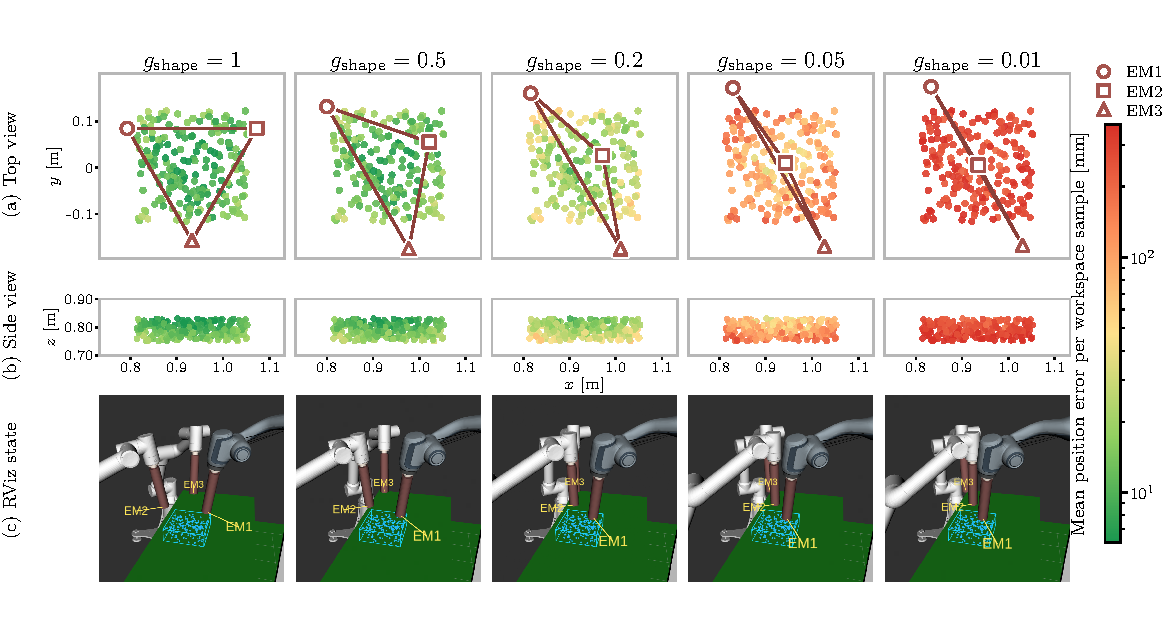
\includegraphics[width=0.96\textwidth,trim=0 18bp 0 24bp,clip]{figures/supp_source_geometry_sequence.pdf}
    \vspace{-0.5\baselineskip}
    \caption[Five representative source geometries and localization results.]{Five representative source geometries and localization results. The columns
    correspond to $g_{\mathrm{shape}}=1$, 0.5, 0.2, 0.05, and 0.01. From top
    to bottom, the rows show (a) top views of the source positions and target samples
    colored by mean position error, (b) side views over the displayed $0.70$--$0.90~\si{\meter}$
    height range, and (c) the corresponding RViz configurations. Circle,
    square, and triangle markers distinguish the three electromagnets.}
    \label{fig:supp_source_geometry_sequence}
\end{figure*}

\begin{table}[htbp]
\centering
\footnotesize
\caption{Localization error across the five representative source geometries.}
\label{tab:supp_source_geometry_results}
\setlength{\tabcolsep}{3pt}
\renewcommand{\arraystretch}{1.1}
\begin{tabular}{ccccc}
\toprule
$g_{\mathrm{shape}}$ & \shortstack{Mean $e_{\bm p}$\\{[mm]}} & \shortstack{Median\\{[mm]}} & \shortstack{P10--P90\\{[mm]}} & \shortstack{Mean $e_{\bm R}$\\{[deg]}} \\
\midrule
1.00 & 11.76 & 11.06 & 6.24--18.10 & 2.93 \\
0.50 & 13.96 & 12.90 & 7.54--22.20 & 3.41 \\
0.20 & 26.85 & 23.68 & 13.55--44.00 & 5.78 \\
0.05 & 109.11 & 99.62 & 51.26--186.72 & 22.43 \\
0.01 & 290.56 & 289.04 & 218.60--368.13 & 68.11 \\
\bottomrule
\end{tabular}
\end{table}
\begin{figure*}[!b]
    \centering
    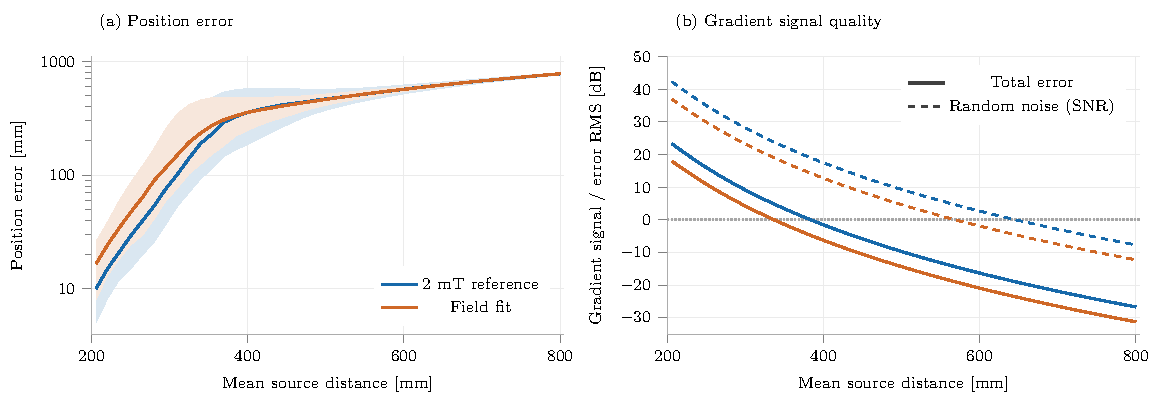
\includegraphics[width=0.88\textwidth,trim=0 4bp 0 6bp,clip]{figures/supp_distance_extension.pdf}
    \vspace{-0.3\baselineskip}
    \caption[Position error and gradient signal quality versus source distance.]{Controlled distance simulation. Colors distinguish the \SI{2}{\milli\tesla} reference and field-fit moment settings. (a) Median position error with 10th--90th percentile bands over 200 realizations. (b) Gradient signal to total error ratio (solid) and random noise SNR (dashed). The horizontal axis is the mean of the three source-to-array distances.}
    \label{fig:supp_distance_extension}
\end{figure*}

\section{Source Distance and Gradient Resolvability}
\label{sec:supp_distance}

\subsection{Controlled Distance Simulation}

We simulate point dipoles using the source positions and tracked magnetic axes averaged over the Fig.~6 poses and the eight-sensor Config.~2 geometry. From a recorded pose, the array moves away along the source-plane normal with fixed orientation, increasing all three source distances over 41 positions (mean distance: \SIrange{205.9}{800}{\milli\meter}). Two fixed moment settings are used: $94.684~\mathrm{A\,m^2}$ per source, giving a mean field magnitude of \SI{2}{\milli\tesla} over the reference poses, and $53.748$, $46.685$, and $65.243~\mathrm{A\,m^2}$ fitted to field vectors from five chronological records.

Each setting uses 200 realizations of static CV measurements with three excitation slots and one shared background slot. Each realization is solved using one measurement per sensor per time slot. We assume independent Gaussian noise of \SI{0.3}{\micro\tesla} standard deviation per sensor axis in each slot. After background subtraction, each source receives an effective residual field discrepancy with zero spatial mean and a vector RMS of \SI{6}{\micro\tesla} across sensors. Noise and residual draws are reused across distances and moment settings. We quantify gradient signal quality by the signal to total reconstruction error ratio
\begin{equation}
    20\log_{10}
    \frac{\sqrt{\sum_{k=1}^{3}\|\bm X_k\|_F^2}}
    {\sqrt{\frac{1}{200}\sum_{t=1}^{200}\sum_{k=1}^{3}
    \|\hat{\bm X}_{k,t}-\bm X_k\|_F^2}}.
    \label{eq:supp_gradient_signal_error_ratio}
\end{equation}
Here $\bm X_k$ is the exact dipole gradient at the array center and $\hat{\bm X}_{k,t}$ is its estimate in realization $t$. The total error includes slot noise, residual discrepancy, and the finite-array approximation. For random noise SNR, the denominator is replaced by the RMS gradient error from slot noise alone.



Both moment settings show increasing position error and decreasing gradient signal quality with distance (Fig.~\ref{fig:supp_distance_extension}). For the \SI{2}{\milli\tesla} reference, increasing the mean distance from \SI{205.9}{\milli\meter} to \SI{399.0}{\milli\meter} raises the median position error from \SI{10.0}{\milli\meter} to \SI{354.4}{\milli\meter} and lowers the gradient signal to total error ratio from \SI{23.3}{\decibel} to \SI{-1.5}{\decibel}. At \SI{800}{\milli\meter}, the random noise SNR falls to \SI{-7.7}{\decibel}. These results show how gradient attenuation relative to the prescribed measurement errors amplifies position error.










\twocolumn[{%
\begin{minipage}{\textwidth}
\section{Motion Artifacts under Sequential Sampling}
\label{sec:supp_tdm_motion}

\begingroup
    \centering
    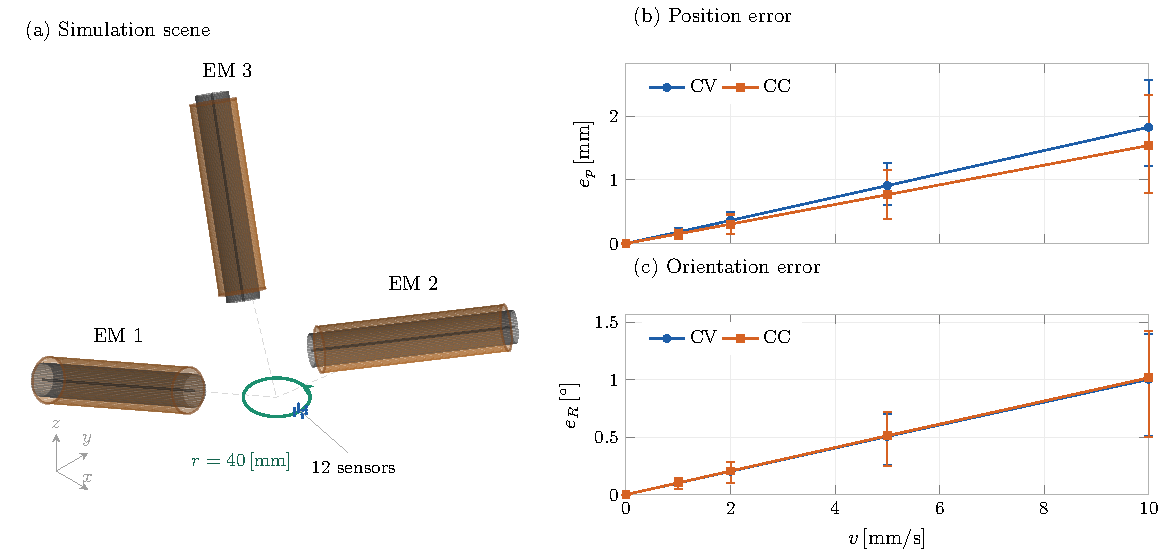
\includegraphics[width=0.9\textwidth]{figures/supp_tdm_motion.pdf}
    \captionof{figure}[Motion artifacts versus translation speed under nominal TDM sampling.]{Noiseless point-dipole simulation with the 12-sensor configuration and source geometry from Fig.~6. (a) Circular translation of radius 40~mm with fixed array orientation. Sensor spacing is enlarged for visibility. (b) Position error and (c) orientation error for CV and CC sampling. Markers show means and error bars span the 5th--95th percentiles over 180 matched trajectory phases at each speed. The nominal CV/CC slot durations are 72/32~ms, with cycle periods of 288/96~ms. Each sensor is sampled at the midpoint of its successive 1~ms window. Errors are referenced to the end of the last active-source acquisition window.}
    \label{fig:supp_tdm_motion}
\endgroup

\newcolumntype{L}[1]{>{\raggedright\arraybackslash}p{#1}}
\newcolumntype{C}[1]{>{\centering\arraybackslash}p{#1}}
\begingroup
\captionof{table}[Comparison of magnetic localization methods.]{Qualitative requirements and reported performance of representative magnetic localization methods.}
\label{tab:draft_literature_comparison}
\centering
\scriptsize
\newcommand{\greencmark}{\textcolor{green!50!black}{\ding{51}}}
\newcommand{\redxmark}{\textcolor{red!75!black}{\ding{55}}}
\newcommand{\spadesym}{\ensuremath{\spadesuit}}
\newcommand{\heartsym}{\textcolor{red}{\ensuremath{\heartsuit}}}
\newcommand{\clubsym}{\ensuremath{\clubsuit}}
\newcommand{\diamondsym}{\textcolor{red}{\ensuremath{\diamondsuit}}}
\newcommand{\quadrantmark}[1]{\textsuperscript{#1}}
\setlength{\tabcolsep}{2.2pt}
\renewcommand{\arraystretch}{1.25}
\newlength{\comparisonwidth}
\setlength{\comparisonwidth}{\dimexpr\textwidth-24\tabcolsep\relax}
\setlength{\comparisonwidth}{1.154734411\comparisonwidth}
\begin{tabular}{L{0.100\comparisonwidth}C{0.035\comparisonwidth}C{0.045\comparisonwidth}C{0.065\comparisonwidth}C{0.048\comparisonwidth}C{0.053\comparisonwidth}C{0.110\comparisonwidth}L{0.105\comparisonwidth}C{0.090\comparisonwidth}C{0.085\comparisonwidth}C{0.070\comparisonwidth}C{0.060\comparisonwidth}}
\hline
\rowcolor{gray!15}
Reference & DoF & Val. & \shortstack{Map-\\free$^\dagger$} & \shortstack{Init.-\\free} & \shortstack{Iter.-\\free} & \shortstack{Source\\requirement} & \shortstack{Workspace/\\envelope} & \shortstack{$e_p$\\(mm)} & \shortstack{$e_R$\\(${}^\circ$)} & \shortstack{$t_{\rm solve}$\\(ms)} & \shortstack{$f_{\rm sys}$\\(Hz)} \\
\hline
Fischer \mbox{\cite{fischerUsingMagneticFields2022}\quadrantmark{\clubsym}}
& 2 & Exp. & \redxmark & \redxmark & \redxmark & 8 EM
& 25-mm local & $2.74$--$7.94$ & -- & $38.3^{a}$ & $10^{a}$ \\
\hline
Fischer \mbox{\cite{fischerGradiometerBasedMagneticLocalization2023}\quadrantmark{\spadesym}}
& 6 & Sim. & \redxmark & \redxmark & \redxmark & 8 EM
& 20--30-mm local & $3.15\pm1.62$ & $3.67\pm3.65$ & NR & NR \\
\hline
Di Natali \mbox{\cite{dinataliJacobianBasedIterativeMethod2016}\quadrantmark{\clubsym}}
& 6 & Exp. & \redxmark & \redxmark & \redxmark & 1 PM
& 150-mm cyl. & $<7$ & $\leq5$ & $1^{b}$ & $>100^{b}$ \\
\hline
von Arx \mbox{\cite{arxSimultaneousLocalizationActuation2023}\quadrantmark{\diamondsym}}
& 6 & Exp. & \redxmark & $\triangle$ & \redxmark & 3 EM
& $80\!\times\!80\!\times\!60$ mm & $0.27$--$0.58$ & $0.48$--$1.83$ & NR & $\leq10$ \\
\hline
Xiang \mbox{\cite{xiangPortableFlexibleIntermediary2026}\quadrantmark{\diamondsym}}
& 6 & Exp. & \redxmark & \greencmark & \redxmark & $\geq4$ poses
& NR & $0.12/0.17^{c}$ & $0.18/0.26^{c}$ & NR & NR \\
\hline
\textbf{GELS}\quadrantmark{\heartsym}
& 6 & Exp. & \greencmark & \greencmark & \greencmark & $\geq3$ EM
& $274\!\times\!175\!\times\!10$ mm & $3.07^{d}$ & $3.79^{d}$ & $0.172$ & $3.47$--$14.49$ \\
\hline
\end{tabular}
\vspace{2pt}
\parbox{\textwidth}{\scriptsize \textbf{Quadrant}: \spadesym~static field + gradiometer; \heartsym~dynamic field + gradiometer; \clubsym~static field + magnetometer; \diamondsym~dynamic field + magnetometer. For a multistage method, the symbol denotes the stage compared in the table. \greencmark: property satisfied; \redxmark: property not satisfied; $\triangle$: not clearly specified; \textbf{NR}: not reported. $^\dagger$\textbf{Map-free}: no pre-calibrated workspace field map or identified source field model or parameters. \textbf{Init.-free}: no externally supplied initial pose estimate is required; an internally generated initializer is allowed. \textbf{Iter.-free}: no online iterative pose optimization. \textbf{Source requirement}: the physical source count and, where needed, the source poses or motion used by the localization procedure. $^{a}$Position-estimation time and sensor sampling rate; computing a new field and gradient setting required $579$ ms. $^{b}$The localization algorithm required $1$ ms, while the full acquisition and communication cycle required $7$ ms. $^{c}$The paper reports no stand-alone NSS initialization error. The listed values are post-L-M patch and internal-magnet errors, respectively, and the latter uses sensor poses returned by the first-stage L-M optimization. $^{d}$Independently best sequence-level GELS values in Fig.~6; they occurred in different Config.~2 CC sequences. Across the six configuration/mode settings, the sequence-level means were $10.80$--$15.57$ mm and $11.5^\circ$--$19.9^\circ$.}
\endgroup

\end{minipage}
}]

\balance
\input{references.bbl}

\end{document}
